\chapter{Proposed System} 
\label{chap3}
%%%%%%%%%%%%%%%%%%%%%%%%%%%%%%%%%%%%%%%%

%\section{Overview}
The implementation aspect of this project requires the development of an infrastructure which can be used to fetch and receive location updates and chat messages in real-time and, where supported, use Augmented Reality to show the markers superimposed on the real world. In this chapter, we will talk about the implementation details, the unforeseen problems that we faced during the development phase and how we chose to overcome them. 

%%%%%%%%%%%%%%%%%%%%%%%%%%%%%%%%%%%%%%%%%%%%%%%%%%%%%%%%%%%%%%%%%%
\section{Major Areas}
We will divide our proposed system into major areas according to their functionality and responsibility. This will help us in focusing on a specific problem at a time and explaining it well so that you could understand it better. Following are some of the major functions of our application: 
\begin{enumerate}
    \item User Account Management
    \item Location Tracking
    \item Contacts Management
    \item Contact's Location Markers
    \item Real-time Chat
    \item Augmented Reality
    \item Chat Bot Integration
\end{enumerate}

Now we will discuss each area separately, and show you how we implemented it in our application.

\section{User Account Management}
We have discussed earlier that we will use \textbf{Firebase Authentication} services for user authentication and account registration. Here, we will show the whole process of how we implemented it, and how we are managing the user's account in our database.

\begin{figure}[H]
    \centering
        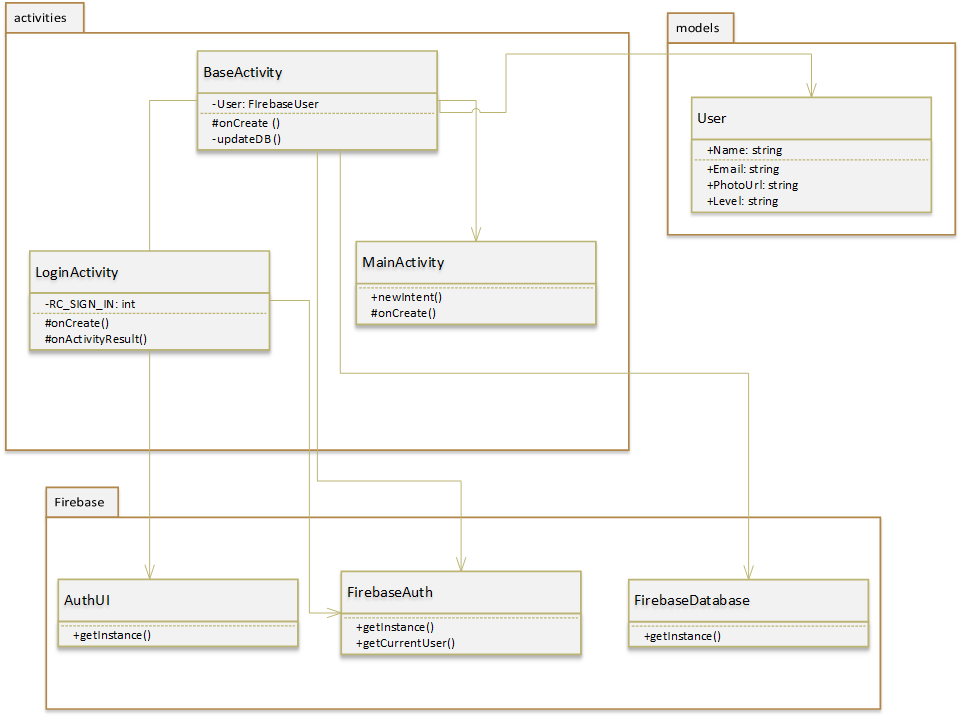
\includegraphics[width=1.00\textwidth]{images/uml-account-login.png}
    \caption{UML for Account Management}
    \label{fig:uml-account-login}
\end{figure}

In Figure \ref{fig:uml-account-login}, we show the UML diagram of the account management system, without going into much detail about other functionality in these classes, just the ones related to the account management. The \texttt{User} class in the \texttt{models} package has private member variables, but with \texttt{getters} and \texttt{setters} for each and every variable, so instead of cluttering the diagram with redundant functions, we have shown them as public member variables here.

As we are developing an Android application, it always starts with a launcher activity. In our case, the launcher activity is the \texttt{BaseActivity}. When the application starts, it launches the \texttt{BaseActivity} and before doing anything else, we see if the user is already logged in. If he is already logged in, we proceed to the \texttt{MainActivity} where the user can freely interact with the application and perform his desired tasks.

However, if the user is not logged in, then we open up the \texttt{LoginActivity}. Here, we use \texttt{FirebaseAuthUI} which is a library developed on top of \textbf{Firebase}. It provides some general functionality regarding account registration and log-in, so we do not have to write much boilerplate code. In \texttt{LoginActivity}, we call the methods of \texttt{AuthUI} to \textit{Register} or \textit{Log in} a user. This opens up a separate screen where the user can register himself for a new account using various options; email-password, Google, Facebook, Twitter, as shown in Figure \ref{fig:khoji_signin}.

Upon registering, the Firebase Authentication saves the credentials of the user in the cloud and returns the user details to our application. We relaunch the \texttt{BaseActivity} class and save the details of the user in our \textbf{Firebase Database} as well, using \texttt{updateDB()} function, because we will be using that throughout the application.

The user details that were returned by the Firebase Authentication also contain a unique identifier for that user, \texttt{uid}. We use that \texttt{uid} to create a new node in the Firebase Database under \texttt{users} node. Now, we have a unique way of referring to that user whenever we want.

After storing the credentials of the user in the Firebase Database, we forward him to the \texttt{MainActivity} where he can carry out his usual tasks.

\begin{figure}[H]
	\centering
		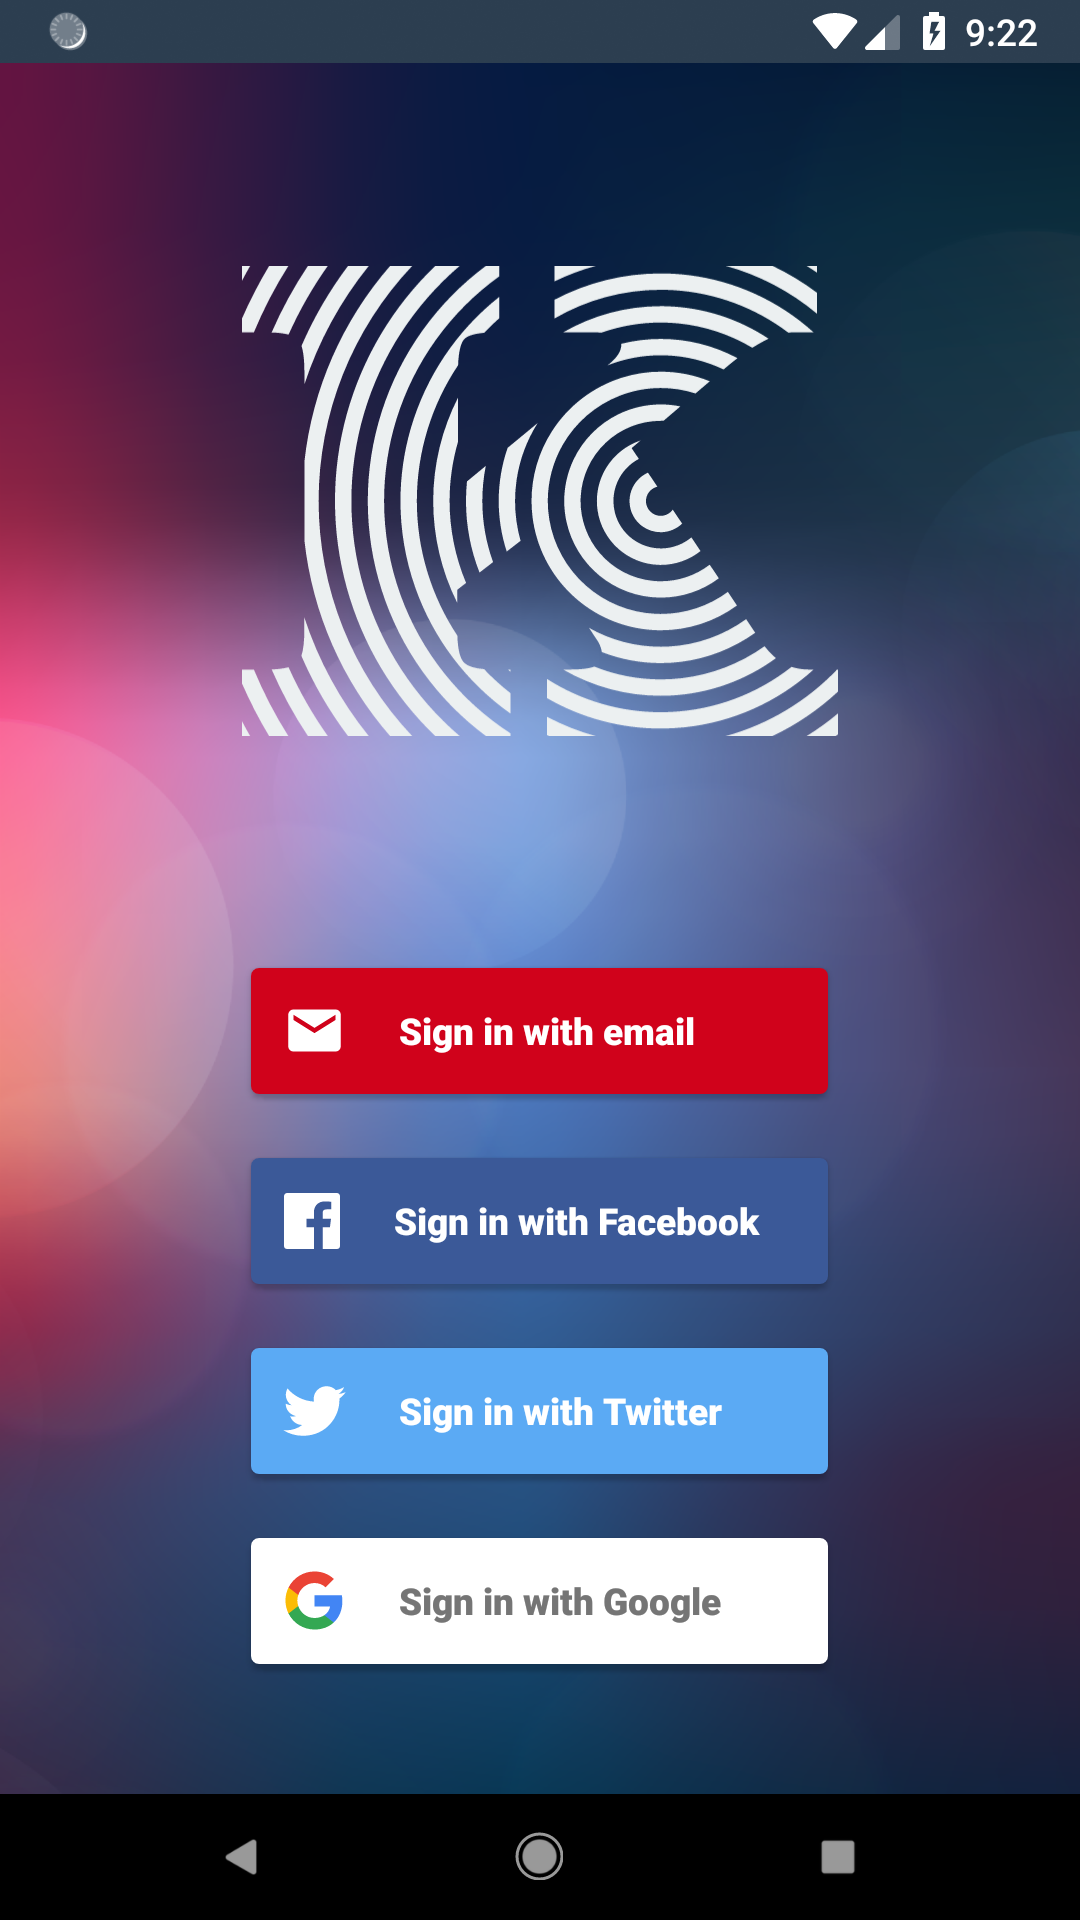
\includegraphics[width=0.80\textwidth]{images/khoji_signin.png}
	\caption{UI for the sign-in screen}
	\label{fig:khoji_signin}
\end{figure}


\section{Location Tracking}
After the user has logged in, the first thing that needs to be done is to start a Location Service, which runs in the background and periodically send updates to his location.

When we started working on this problem, before the release of Android 8.0 (API level 26), the way to solve this problem was entirely different. Before Android 8.0, we could query for Location updates as frequently as we wanted to. The API for listening to Location updates was also quite simple as compared to what it is now. 

However, midway into developing this application, Android 8.0 was released which changed the way to retrieve location quite radically. They limited how frequently background apps can retrieve the user's current location \cite{GoogleLocationLimits2018}. When the app was in the foreground, we could ask for location updates as frequently as wanted, but when it was running in the background, we could not. We had to query for location update to the Android system, and it would only return the update only a few times each hour, no matter how frequently we requested it.

Because of this limitation, we had to redesign our whole app, keeping in mind the limitations imposed by the new standards as well as the new API that was recommended for this. Now, when the app is in foreground, that is the user is actively interacting with it, we use a different location retrieval logic which asks for location updates every few seconds. However, when the app goes to the background, we start a background Job service, which updates the location every few times in an hour. We do not have much of a control over how frequent the updates will be in the background as the Android OS takes it in his own hands to handle background services so as to increase the battery performance of the system.

As shown in Figure \ref{fig:uml-location}, in \texttt{MainActivity} we start listening for location updates. This will listen to the location updates in the foreground, and as soon as we receive an update, it will store that location in the Firebase Database under the \texttt{locations} node. The \texttt{uid} will store each location of the currently logged in user. \texttt{UserLocation} class is used to model the location and storage and retrieval of the location for the database. Again, the public member fields shown in the figure are not public, they are \textbf{private} but with getter and setter methods.

\begin{figure}[H]
    \centering
        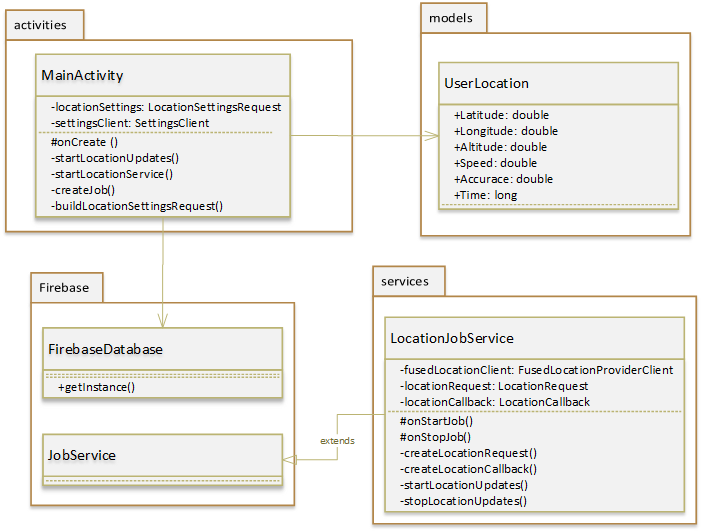
\includegraphics[width=1.00\textwidth]{images/uml-location.png}
    \caption{UML diagram for Location Tracking}
    \label{fig:uml-location}
\end{figure}

We start location service in the \texttt{MainActivity} as well, which start the background service for listening to the location updates. It creates a \texttt{LocationJobService}, which \texttt{extends JobService} which runs in the background and whenever it receives a location update, it updates it in the database.

There is also boilerplate code present for requesting location tracking permissions, following best practices for Android 6.0 and higher \cite{AndroidPermissions2018}. In \texttt{MainActivity}, we also keep track of whether the user has enabled the location service on his device or is it turned off. If it is turned off, we prompt him to enable the location service, as shown in Figure \ref{fig:khoji_location_permission}, so he could use the app effectively.

\begin{figure}[H]
	\centering
		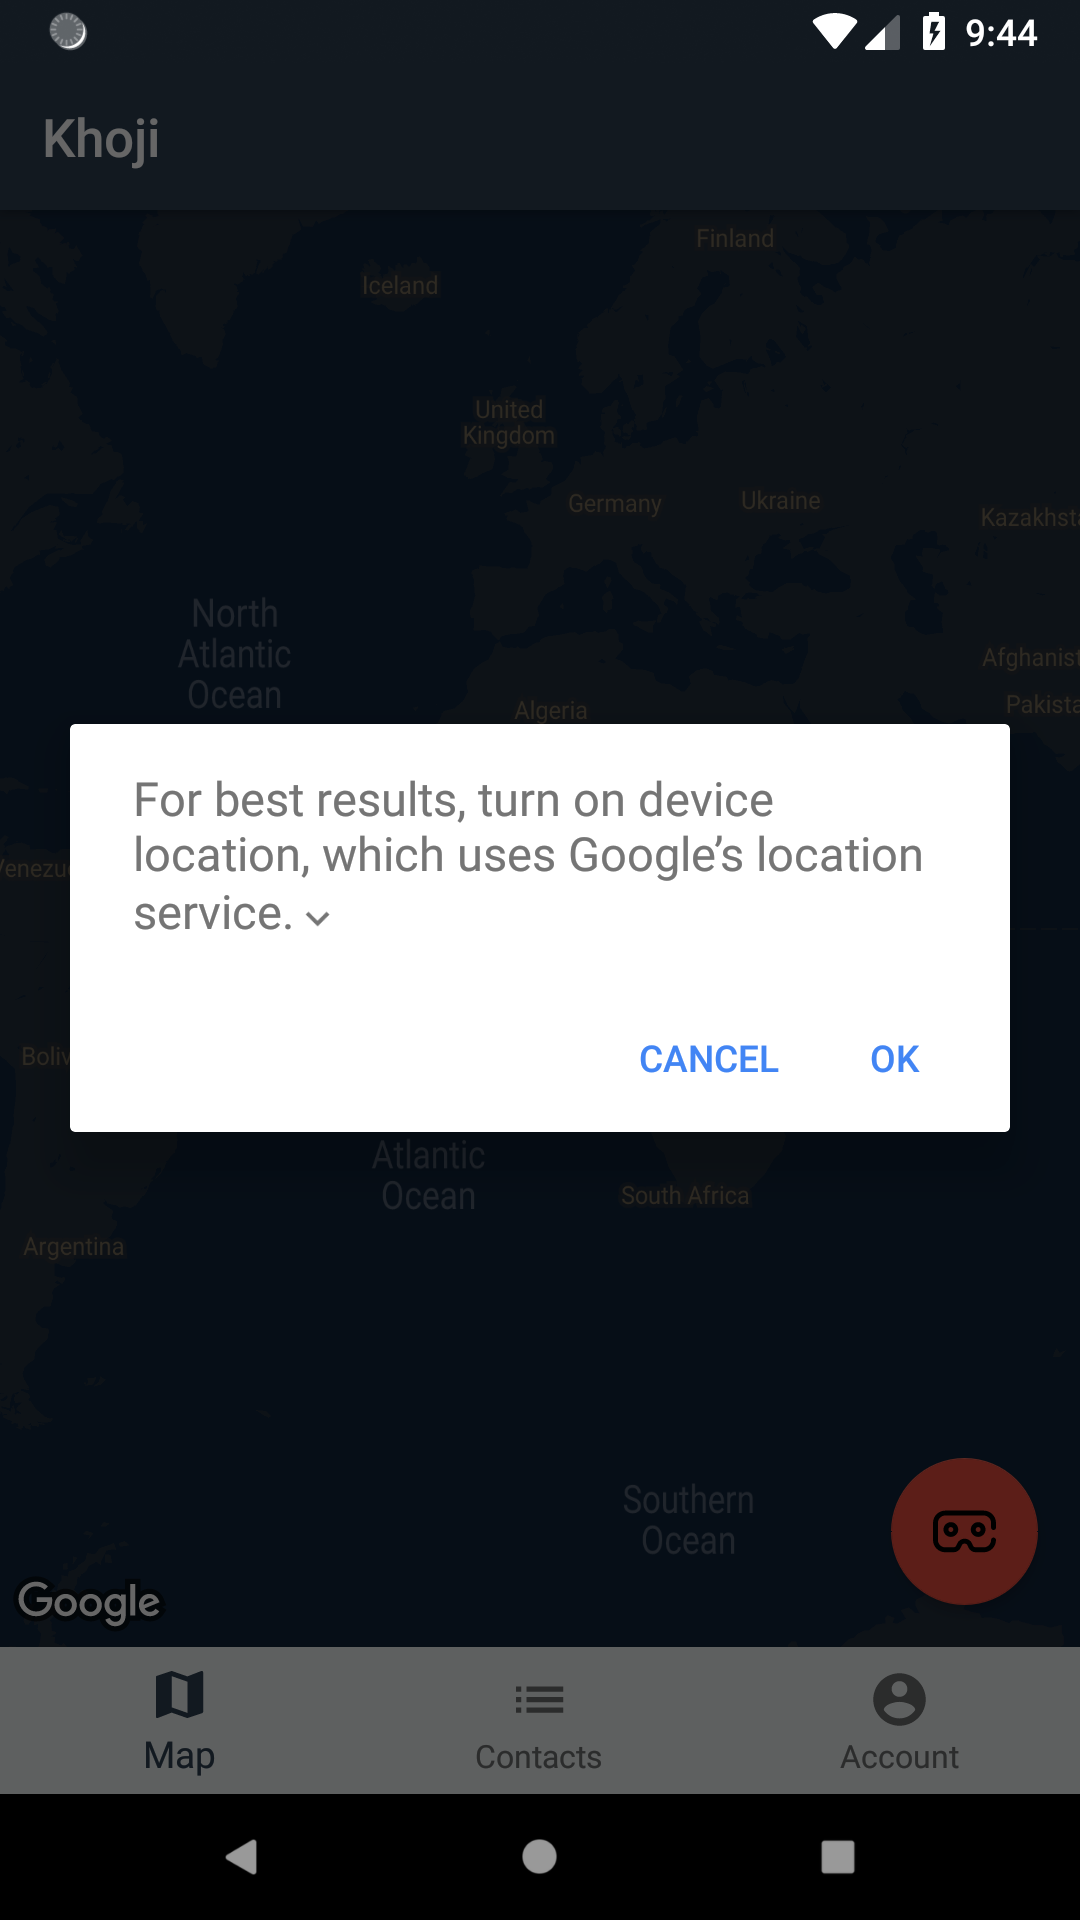
\includegraphics[width=0.80\textwidth]{images/khoji_location_permission.png}
	\caption{UI for enabling the location permission, if disabled}
	\label{fig:khoji_location_permission}
\end{figure}



\section{Contacts Management}
Another best practice in Android development is to use \texttt{Fragments}. Fragments represent a behavior or a portion of the user interface in an activity. They are always hosted inside an Activity, and when that activity is closed or gets destroyed, they are also destroyed along with it. Fragments increase the modularity and re-usability of the application \cite{AndroidFragments2018}.

We have made use of fragments in our application extensively. \texttt{MainActivity} acts as a placeholder for different fragments. When the user presses a button to change screen, the \textbf{fragment container} in the \texttt{MainActivity} gets updated so that the old fragment is replaced with the new fragment in the container. This helps in keeping the code modular and making the user interface responsive.

\begin{figure}[H]
    \centering
        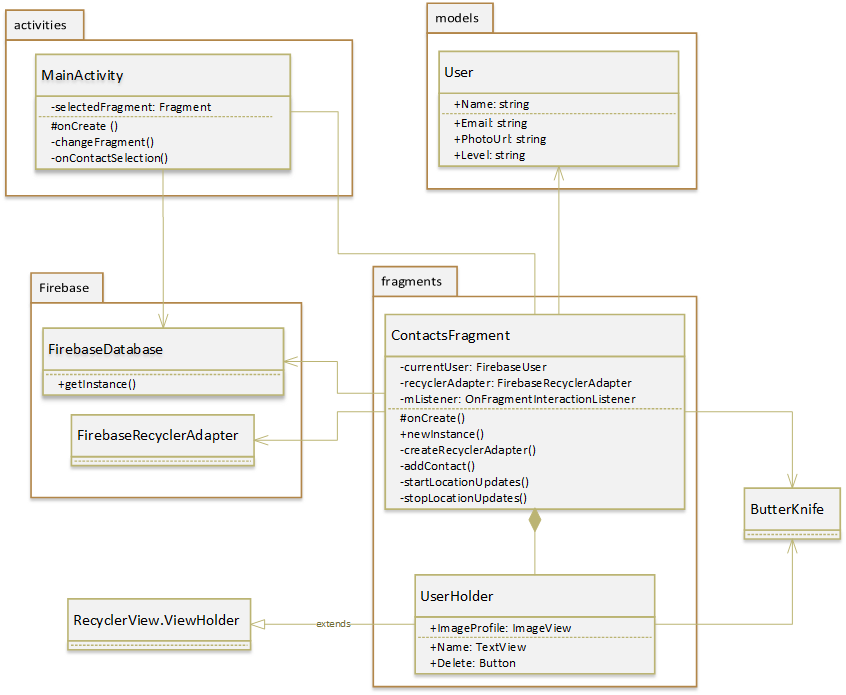
\includegraphics[width=1.00\textwidth]{images/uml-contacts.png}
    \caption{UML diagram for Contacts Management}
    \label{fig:uml-contacts}
\end{figure}

As shown in Figure \ref{fig:uml-contacts}, when the user presses the button to change the fragment to \texttt{ContactsFragment}, we update the fragment container in the \texttt{MainActivity} to load \texttt{ContactsFragment}. In ContactsFragment, the user can see the list of all of his contacts, remove the ones he does not need anymore and add additional contacts to his contact list. 

To add a new contact to his contact list, a user must type the email address of the user that he wants to add. If the email address is present in the database, then that contact will be added to his contact list, and the contact list of both the users will be updated to show the newly added contacts.

We use \texttt{FirebaseRecyclerAdapter} to populate the list of all the contacts a user have. This class automatically fetches the list of contacts from the Firebase Database, maps them into \texttt{User} class and populates the \texttt{RecyclerView} with the layout that we specify in the options. This reduces much boilerplate code.

Another library that we use heavily throughout the project is \texttt{ButterKnife}. This library binds the views from the layout files to the java source code files so we could easily access them in the code. By using this library, we do not have to type out a whole lot of redundant code as it has been taken care of by this library.

\texttt{UserHolder} class is an inner class of ContactsFragment which only holds the views that need to be populated in the list once the data is retrieved from the database. This class extends \texttt{RecyclerView.ViewHolder} class and we use \texttt{ButterKnife} to bind the views from the layout file to the field variables.

The user interface for the contacts management is shown in Figure \ref{fig:khoji_contacts}. To add a new user to the contact list, one must have to add the email address of the user that he wants to add in the field marked by \textbf{1} and then press the add contact icon, marked by \textbf{2} in the image. If the user is available in the system, he will be added to the contacts list of the current user and the list shown below will be updated immediately to reflect the new addition.

By clicking on the user name or user image in the list, as shown by the marking \textbf{3} in the figure, the current user will be taken to the location marker of that contact in the Google Maps view. If he clicks on the chat icon, marked by \textbf{4} in the figure, a new chat window will appear so that the user can start chatting with that person. By clicking on the trash icon, marked by \textbf{5} in the figure, the user can remove that person from his contacts list.

\begin{figure}[H]
	\centering
		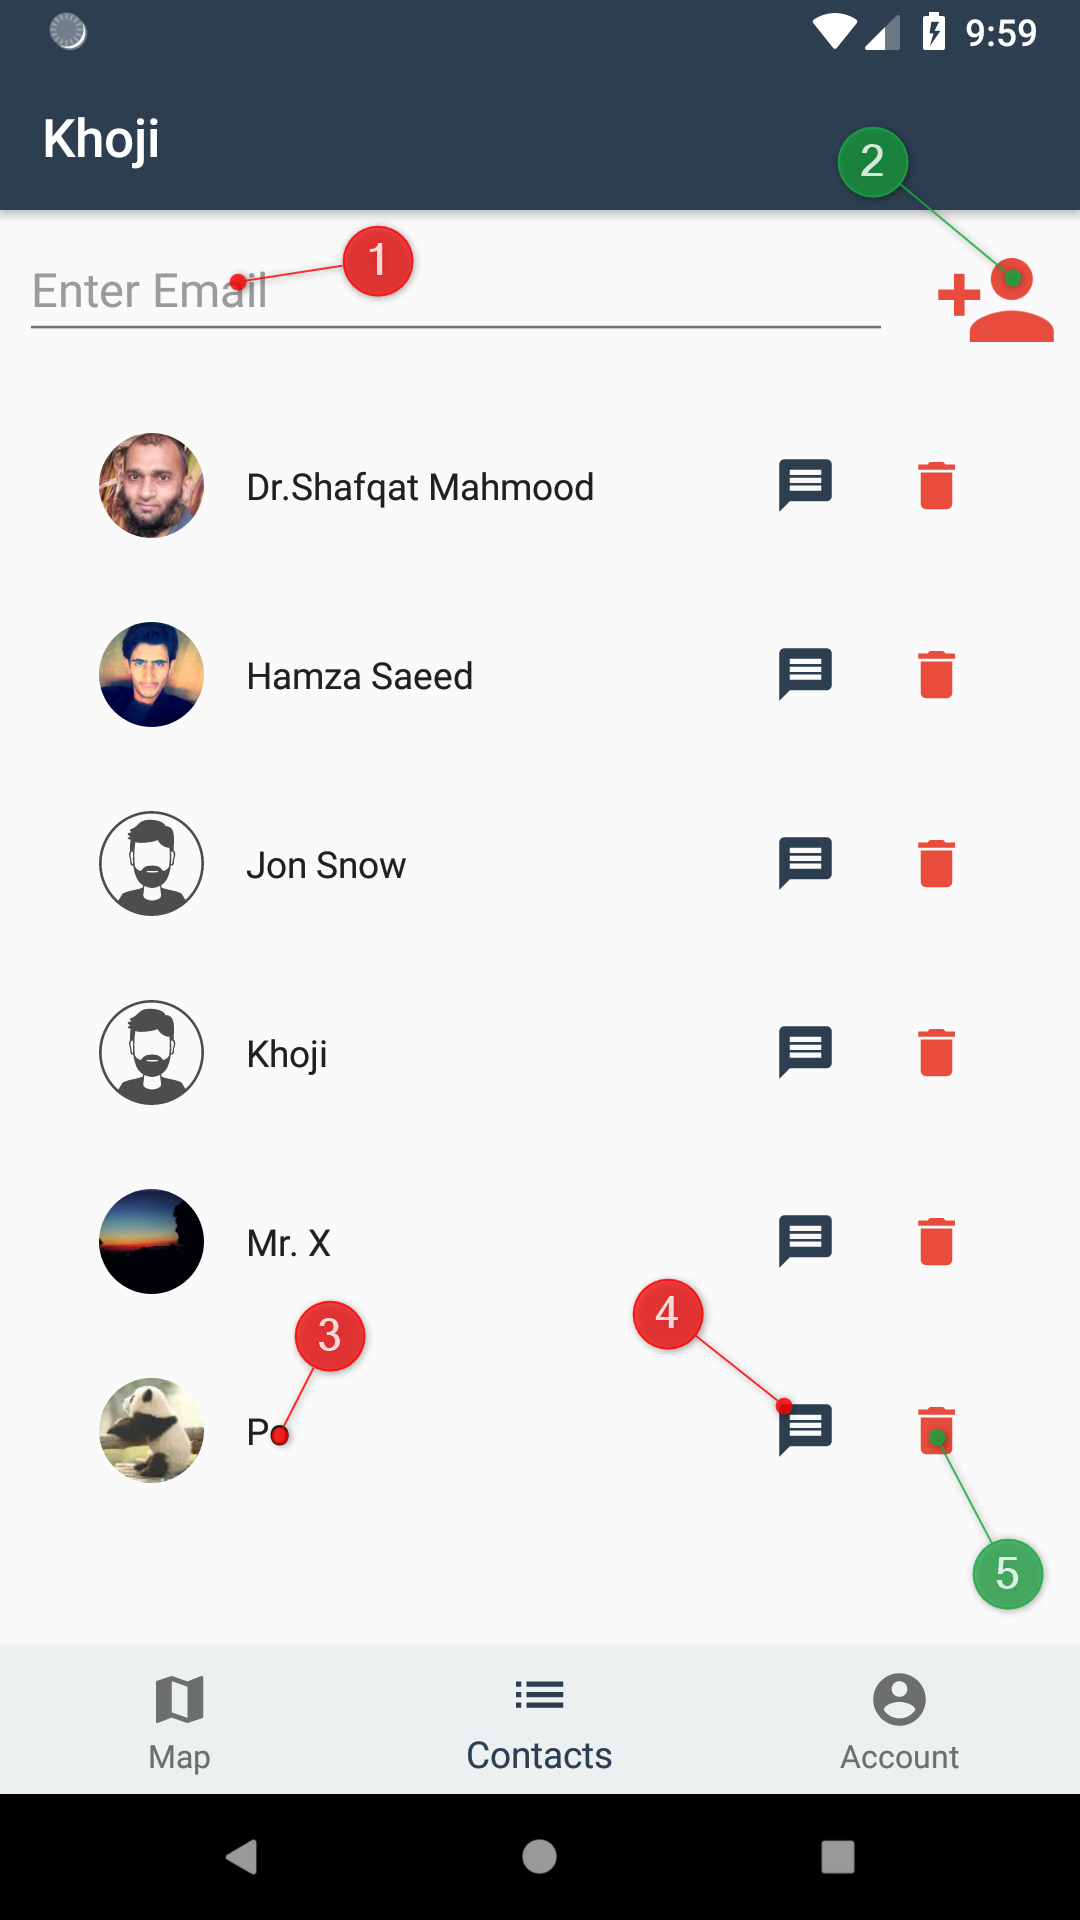
\includegraphics[width=0.65\textwidth]{images/khoji_contacts_1.png}
	\caption{UI for Contact Management screen}
	\label{fig:khoji_contacts}
\end{figure}



\section{Contact's Location Markers}
Now that we have a way to store the location of every user using our app and we have devised a way for users to add one another as each other's contacts, it is time to fetch the location details of each of a user's contact and show them as markers on a map. We are using a map here because we also need to keep in mind the users that don't have devices capable of augmented reality. If we only used augmented reality to visualize the location of users, then it would not have been usable by those that do not have access to an AR-enabled device, and as a result, it would not have been usable by those that do have an AR supported device because they would not be able to add their friends and family as their contacts.

\begin{figure}
    \centering
        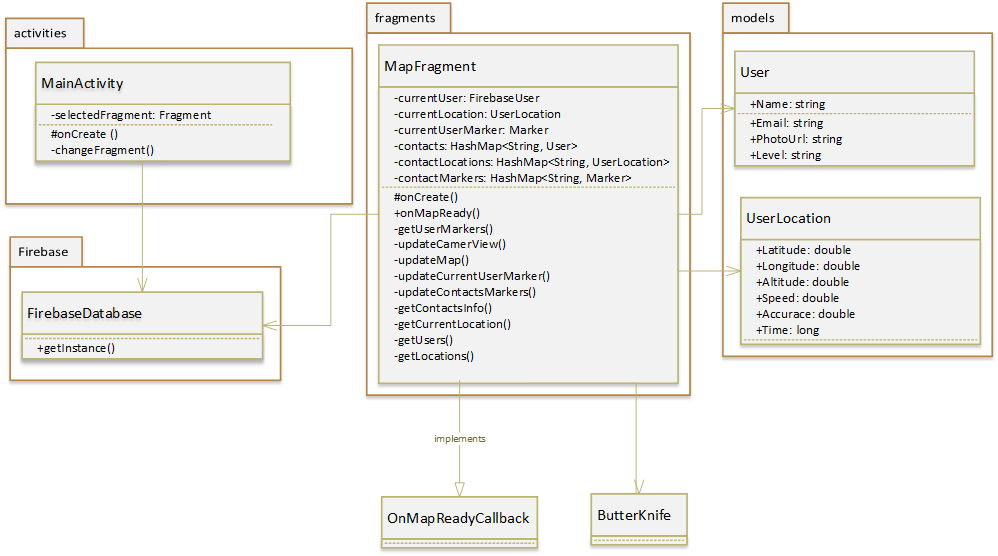
\includegraphics[width=1.00\textwidth]{images/uml-map.png}
    \caption{UML diagram for Contact's Location Markers}
    \label{fig:uml-map}
\end{figure}

As shown in Figure \ref{fig:uml-map}, we load the \texttt{MapFragment} into the fragment container located in the \texttt{MainActivity}. In MapFragment, we use \textbf{Google Maps SDK} to load Google Maps in our view. For this reason, the \texttt{MapFramgent} class \texttt{implements OnMapReadyCallback}, which gets called, as the name suggests, when the map is ready. After Augmented Reality implementation, this was the most cumbersome and difficult implementation in the whole project, as we had to keep track of many things and infuse multiple technologies together.

\texttt{MapFragment} class keeps track of the current location of the logged in user and updates his marker on the map, which is shown in green on the map to distinguish him from his contact's markers. \texttt{MapFragment} class then queries the Firebase Database to retrieve the contacts of that user. This query will return only the \texttt{uid} and the name of their contacts, as we have designed the database schema in Section \ref{data schema} in such a way.  

Now that we have the \texttt{uid}s of the user's contacts, we store them in a list and query the database for \texttt{UserLocation} updates on each and every user in the contact list. We store them in a \texttt{HashMap} where the key is the \texttt{uid} of the user and the value is the \texttt{UserLocation} class populated with the details of that particular user. We also query for the user information for each user in the contact list and store them in another \texttt{HashMap} where they key is \texttt{uid} of the user and value is the \texttt{User} class populated with the details of that user.

Now that we have all the detail that we need to populate the Map view with user markers, we create a \texttt{HashMap} to store the Markers as well, where again, the key is \texttt{uid} of the user and the value is the \texttt{Marker} for that user. We need to keep track of each marker because when the location of that user changes, we need to update the marker as well to reflect that change. We then populate the Map with all the markers, both the current user's which is shown in green color as well as of contact's markers which are shown in red.

After that, we set-up a \textbf{Firebase Database Listener} that listen to any changes, if they happen in the database. Whenever the location of the user changes, it will trigger an \textbf{event} and we will handle it by fetching the latest location of that user from the database and updating it in our \texttt{HashMap}s as well as on Google Map view.

\begin{figure}
	\centering
		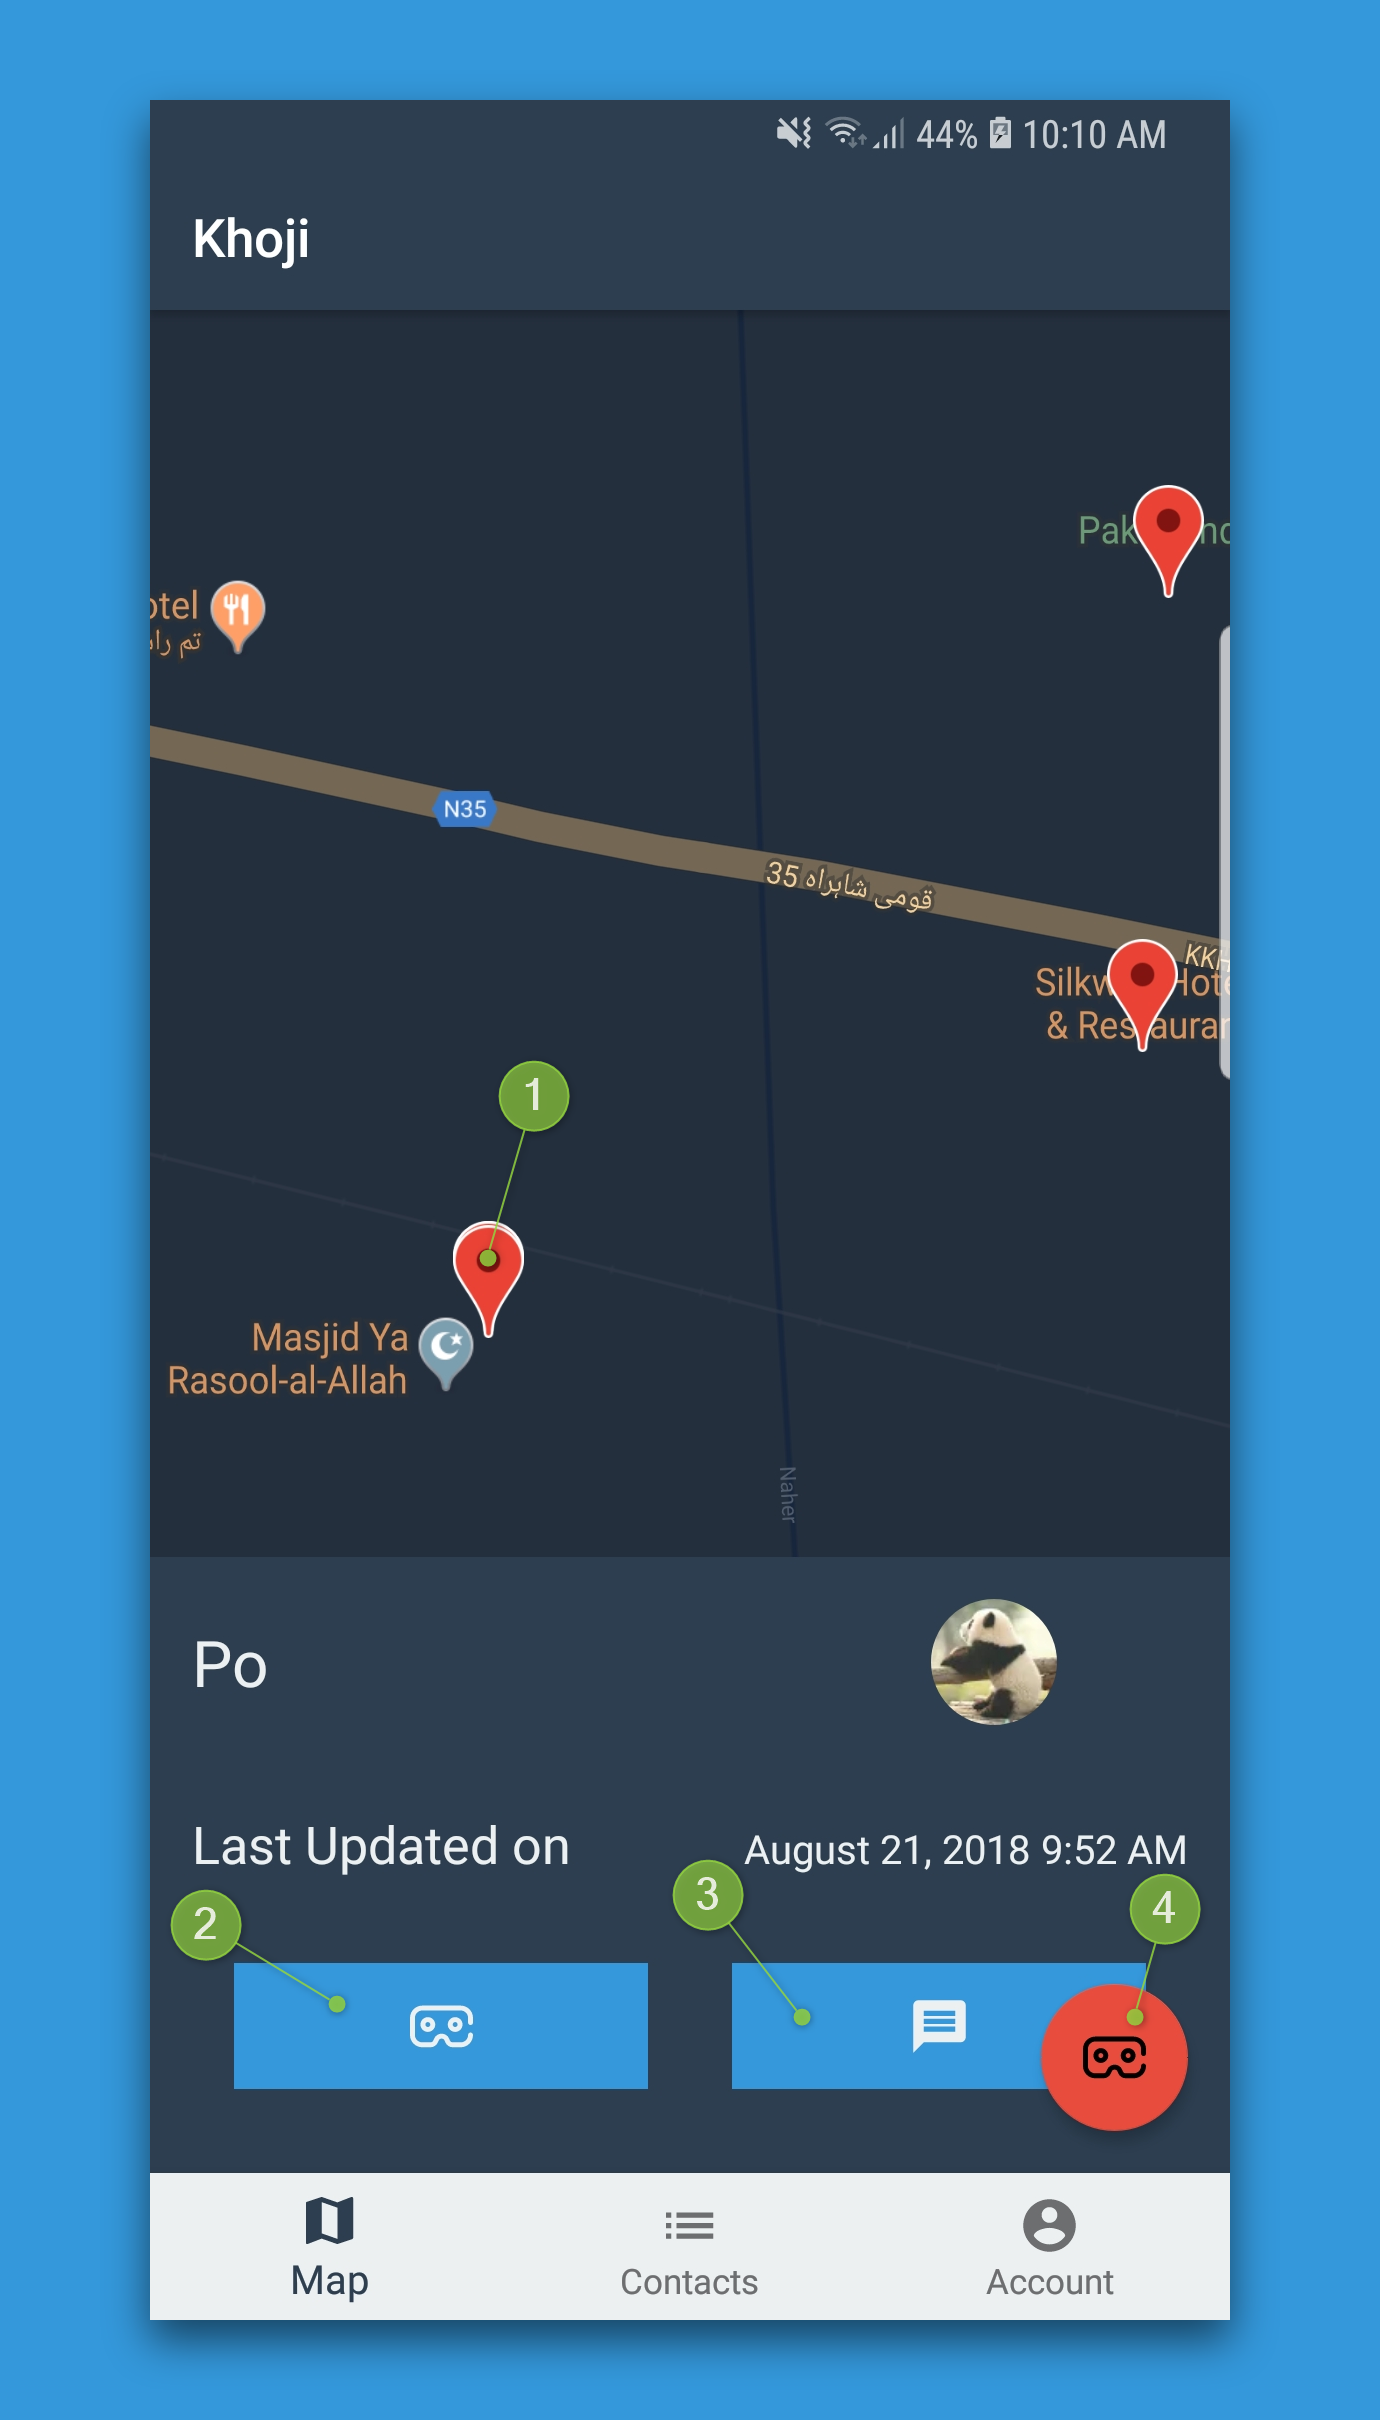
\includegraphics[width=0.80\textwidth]{images/khoji_location_markers_2.png}
	\caption{UI for Location Markers on the map}
	\label{fig:khoji_location_markers}
\end{figure}

As shown in Figure \ref{fig:khoji_location_markers}, when a user clicks on a marker, marked by \textbf{1} in the figure, a small window will show up at the bottom of the screen which will list further information about that marker, e.g. name, last update time etc. along with other operations that could be performed for that marker. If the AR is supported on that device, by clicking on the AR button, marked by \textbf{2} in the figure, the AR activity will be launched which will only show the AR marker of that particular user in the real-world. If the user presses chat icon, marked by \textbf{3} in the figure, then a chat window will appear so he could chat with that user. Finally, by pressing the icon marked by \textbf{4} in the figure, the user can launch AR activity which will show all the markers of the users that are in the contact list of that particular user.




\section{Augmented Reality}
In this section, we will talk about the problems that we faced during the implementation of this feature and the different approaches we used to overcome those problems.
\subsection{Problems}
We faced a lot of problems with the implementation of this feature in our application. The \texttt{ARCore} library was in early beta release when we started working on this problem. So there was little to no documentation available. We had to look at the source code to figure out how the code is supposed to work.

Another main problem was the stability of the AR objects. During beta release of the library, there were a lot of bugs and the stability was quite weak, but with every update, it improved a little bit. However, along with the improvement of the library, the API of the library also changed, and the way to do things was also affected by this. This resulted in code rewrite every time there was an update as the previous code would not work with the new API.

Another main problem is that the ARCore library was not designed with world-scale AR in mind. Now that it has matured enough, it still does not work very well with world-scale AR where we place AR objects in the real-world using longitude and latitude. ARCore works best by scanning a surface and create a cloud of points where a user can place their AR objects, and it anchors that object to that point in the cloud. Because of the cloud of points, we can see the object exactly where we placed. ARCore is perfect for this type of AR, but in our application, we are using world-scale AR which means there are no points of cloud present and we place the object using longitude and latitude. This has serious stability issues, as the marker would keep floating in the AR scene or it could be shown in West while it needed to be in the East.

\subsection{Different Approaches}
During the lifetime of this project, we have tried several approaches to solve the problem of implementing Augmented Reality into our application. It has proven to be a lot more difficult task than we imagined it to be. As with any new technology, the lack of proper documentation and the scarcity of tutorials make it much harder to implement it for our application. Here we will briefly describe some of the things that we tried to make it work for us.

\subsection{Unity and Mapbox}
After completing the functionalities as mentioned above of the application, we looked at several online resources to see what would be the best way for us to implement Augmented Reality into our application. After searching long and hard, we decided to use \textbf{Unity} and \textbf{Mapbox} for this, as they were already working on the problem of world-scale AR and had a library for location-based AR \cite{MapboxUnitySDK2018}. 

We were successful in creating a basic prototype that would fetch results from the Firebase Database and show them in AR using Unity Engine. However, there were some problems with device calibration which resulted in the poor mapping of AR markers to the real-world location. The inner compass of the mobile phone was poorly calibrated to work with it, meaning if the user was in East, the AR environment would show him in West. Another main reason why we decided to abandon that approach is that Unity was not very optimized for Android. It can build a solution for multiple platforms, including Android, iOS, Windows, Oculus, etc. but for Android, we needed to extract every single bit of performance gain that we could get. Before that, we had already implemented the rest of the system architecture in Android, so now, linking a poorly working, resource massive Unity project with our Android app did not seem very efficient. So, we put that aside and tried working with ARCore, using Java.

\subsection{ARCore with OpenGL}
When we started this project, the \textbf{ARCore} library was still in early beta. There was little to no documentation available, and we had to look at source code and one or two available examples on the internet to understand how the library works. This was a very tiresome and unrewarding experience for us. Moreover, at that time, we had to work with \textbf{OpenGL} to render objects onto the AR scene, which itself is quite a tedious task.

After a lot of hard work, we were able to visualize the markers in AR using simple views that just showed the name of the contact. The same problem persisted here. The markers were not stable. They would keep floating in the AR scene view, always trying to adjust their position.

Although we were very frustrated after this, we still did not give up and started our hunt for some other way this problem could be solved.

\subsection{ARCore Location}
At this time, a new open-source library was released on Github.com, ARCore Location \cite{ARCoreLocation2018}, which was trying to solve the same problem that we were having, i.e., placing AR objects within the AR scene with real-world GPS coordinates. We decided to give it a try.

As compared to previous solutions, this was easy for us to implement, because they provided a working example which we can use to understand how this library works. This library also removed a lot of the boilerplate code that we wrote for our previous version. Under the hood, it was doing the same thing that we were doing before, just that it provided a nice API so that we do not have to write all that boilerplate code ourselves.

We integrated this library into our application. At that time, we were still using OpenGL to render AR objects into the AR scene, which is tedious low-level work with graphics and quite exhausting to modify. This made it harder to experiment with different methodologies and techniques as their was always the danger of breaking it all together.

We noticed a little bit of improvement in the stability of the markers but their positioning was still wrong, and after a few seconds, the markers would start floating again. We decided to keep this solution for now, as it refactored and cleaned our code somewhat.

\subsection{Current Approach}
Now, we are using the same library, \texttt{ARCoreLocation} \cite{ARCoreLocation2018}, but we have updated it to the latest release. We started with \textbf{ARCore} when it was in beta, and now, we are using \textbf{ARCore v1.3}. This version is a lot more stable than previous versions. The markers that are shown in the AR scene do not float now. There is a little bit issue with the positioning of the markers sometimes, but mostly it works fine now.

Another significant change in the new version of ARCore was the inclusion of \texttt{SceneForm}. By using this, we do not have to work with 3D graphics and \textbf{OpenGL} at such a low level. \texttt{SceneForm} provides us with a high-level API, realistic physically based renderer for importing, viewing, and building 3D assets and easy integration into ARCore \cite{ARCoreSceneForm2018}.

As you can see in Figure \ref{fig:uml-ar}, the \texttt{ArActivity} is started when the user presses the button from the \texttt{MapsFragment}. If the device of the user supports Augmented Reality, then the button will be enabled; otherwise, it will be disabled. When the \texttt{ArActivity} launches, it first checks if the \textbf{ARCore} library is installed on the user's device. If it is not installed, it prompts the user to install the library. After that, it checks to see if the user has given the necessary permissions for the app to use AR features and prompts the user to do so if he has not given the permission yet.

\begin{figure}
    \centering
        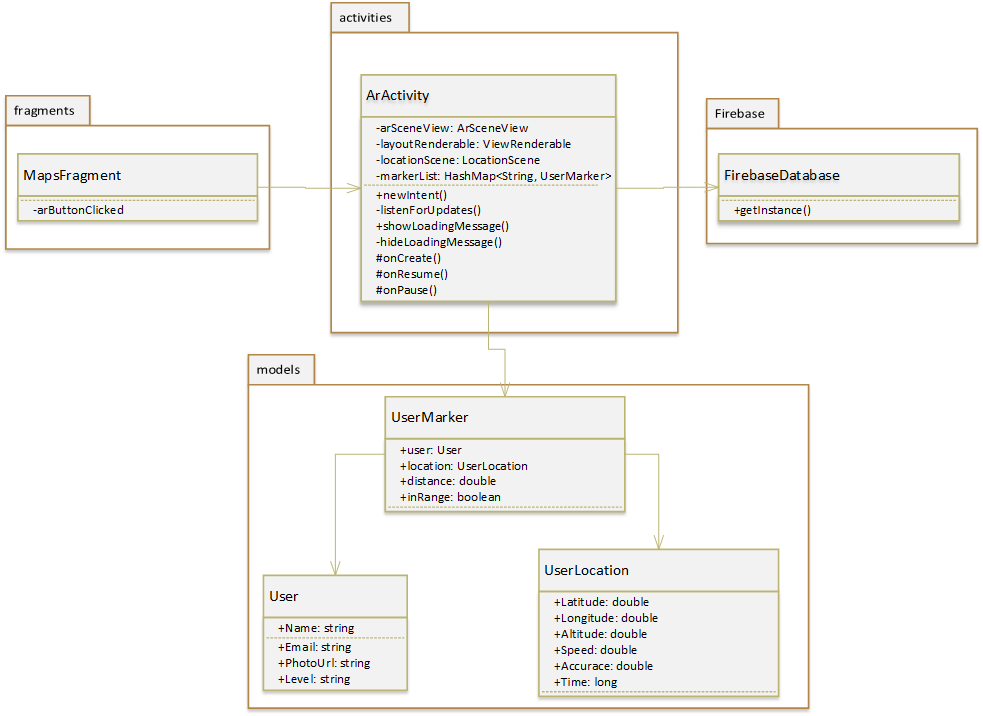
\includegraphics[width=1.00\textwidth]{images/uml-ar.png}
    \caption{UML diagram for AR activity}
    \label{fig:uml-ar}
\end{figure}

Once everything is set-up, the application will then place the markers, loading from the \texttt{HashMap<String, UserMaker>} which was passed to this activity from the \texttt{MapsFragment} class. This will display the markers in the AR scene at their respective GPS coordinates.

The application will also start listening to the changes in the database. As soon as the location of the contact is updated in the database, it will be fetched from the database, and the respective marker will be updated to reflect the new position of the user.

In Figure \ref{fig:khoji_ar_marker}, we can see how the marker will be superimposed on the real-world. Here, it is showing the name, profile picture and the distance of that person from the user at that moment. If the user clicks on the marker, a small window will appear at the bottom, showing further details, like the last time of location update and the option to launch the chat activity so you could start chatting with that person instantly.

\begin{figure}[H]
	\centering
		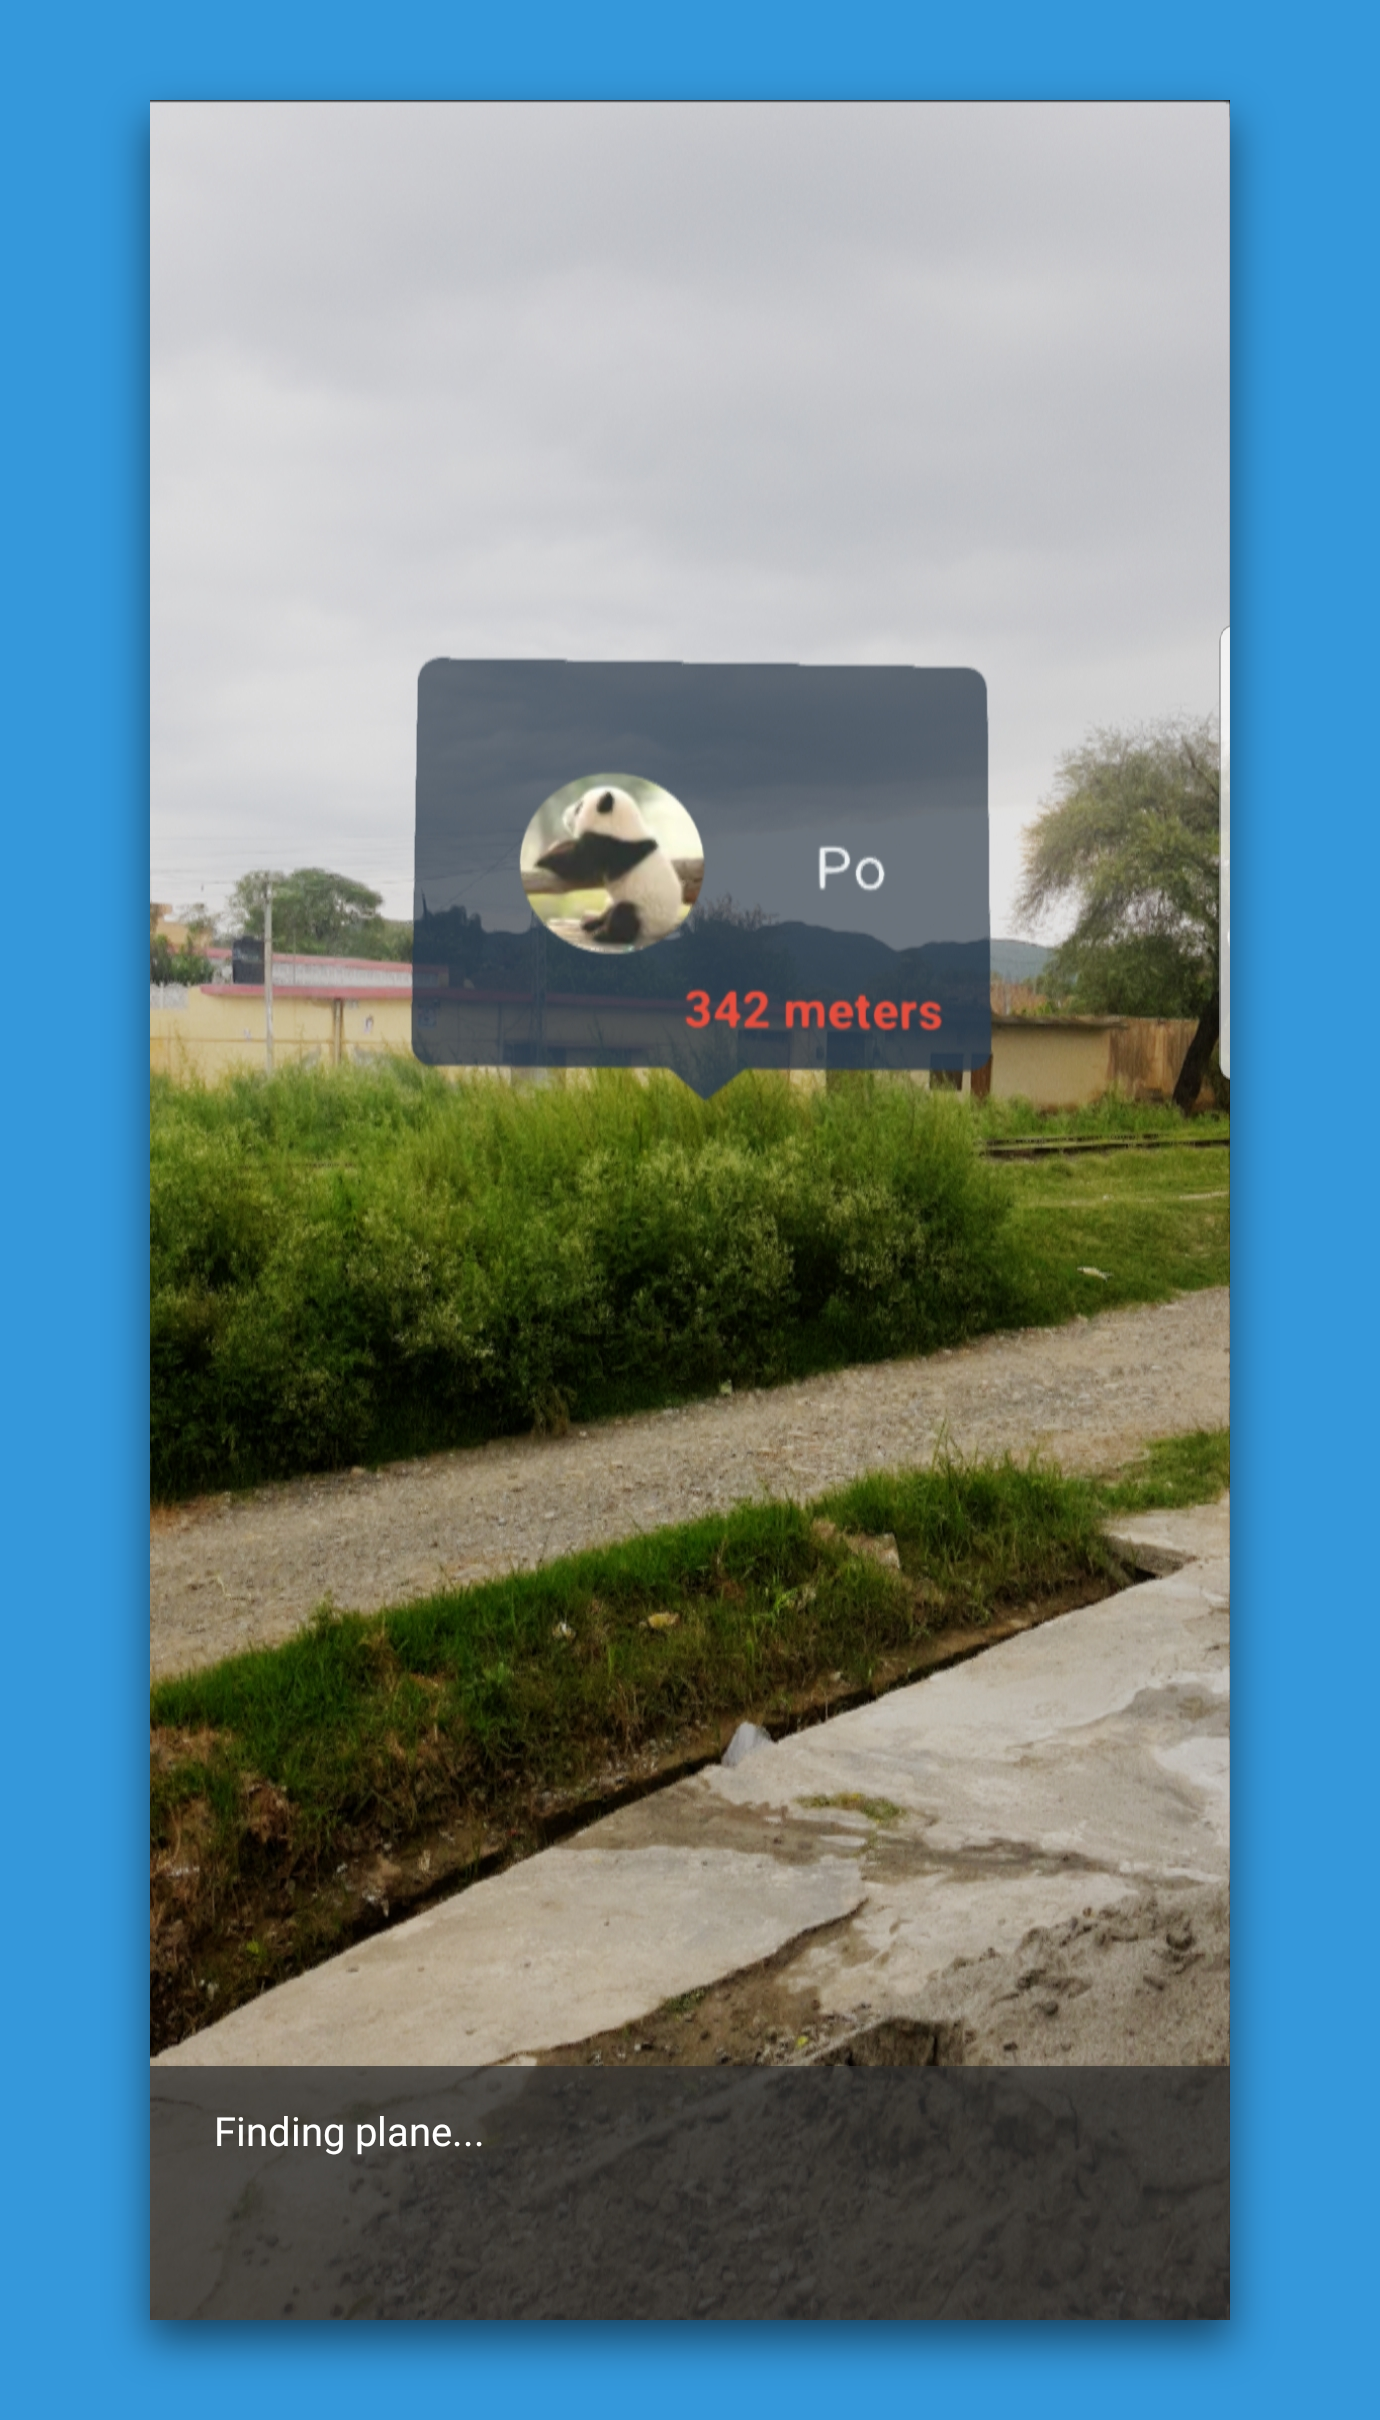
\includegraphics[width=0.80\textwidth]{images/khoji_ar_marker.png}
	\caption{User marker shown in AR}
	\label{fig:khoji_ar_marker}
\end{figure}


\section{Real-time Chat}
We also used the Firebase Database for implementing real-time chatting in our application. When the user presses the chat icon from the \texttt{ContactsFragment} class, it opens up a new activity where he is provided with chatting functionality with his Contact so he could quickly get in touch with him.


\begin{figure}
    \centering
        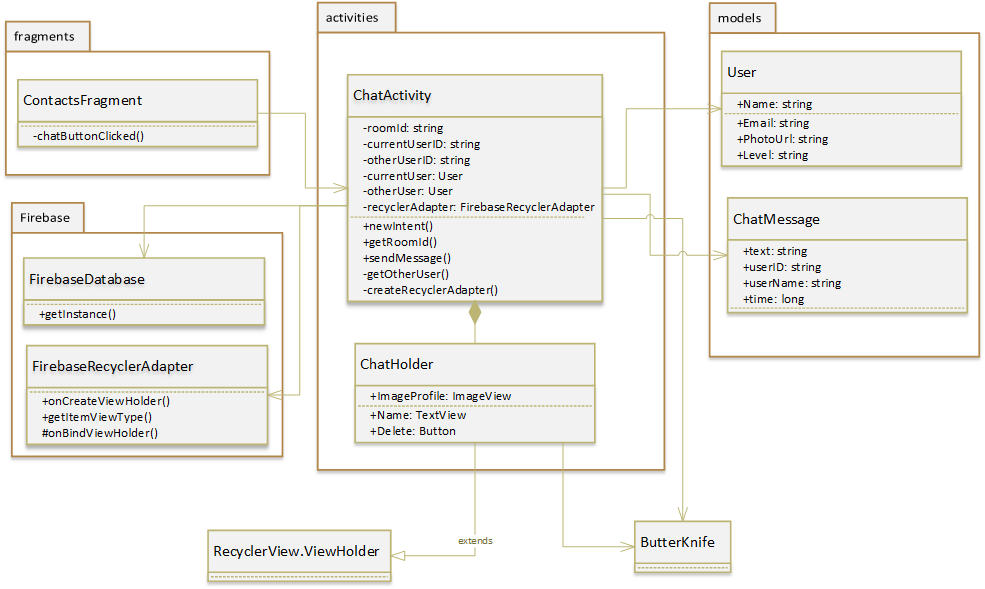
\includegraphics[width=1.00\textwidth]{images/uml-chat.png}
    \caption{UML diagram for Real-time Chat}
    \label{fig:uml-chat}
\end{figure}


We can see, from Figure \ref{fig:uml-chat}, that the \texttt{ChatActivity} class uses two classes from the model package, one \texttt{User} class and the other \texttt{ChatMessage} class. \texttt{User} class is used to retrieve the info of the contact that the currently logged in user wants to talk to. Also, the \texttt{ChatMessage} class is used to read and write chat messages into the Firebase database and show them in the chat message \texttt{RecyclerView} as well.

We have followed the best practice in designing the database schema for chat rooms so that there is no unnecessary cluttering of data and the data is perfectly denormalized. We generate the chat room id using this simple algorithm: 

\begin{verbatim}
public static String getRoomId(String uid1, String uid2) {
  return ((uid1.compareTo(uid2) > 0) ? 
                    uid1 + '_' + uid2 : 
                  uid2 + '_' + uid1);
}
\end{verbatim}

This algorithm will ensure that there will always be a unique room\_id and we can easily query it whenever we want. We are concatenating the \texttt{uid}s of both the users that are participating in that chat room. We use lexicographical order to sort the \texttt{uid}s and then concatenate them.

When a user sends a message, we store the details of the message; \textit{message text, message time, sender id, sender name}; in \texttt{ChatMessage} class and then write that information in the Firebase Database.

To display the chat messages, we use \texttt{FirebaseRecyclerAdapter} which fetches the latest messages from the database and populates the list according to our specified layout. We use a separate layout for different type of messages, that is, for messages sent by the current user and the received messages. We also listen to the database changes, as soon as a new message arrives, we populate the message list with that new message and scroll the list to the latest message position.

\begin{figure}[H]
	\centering
		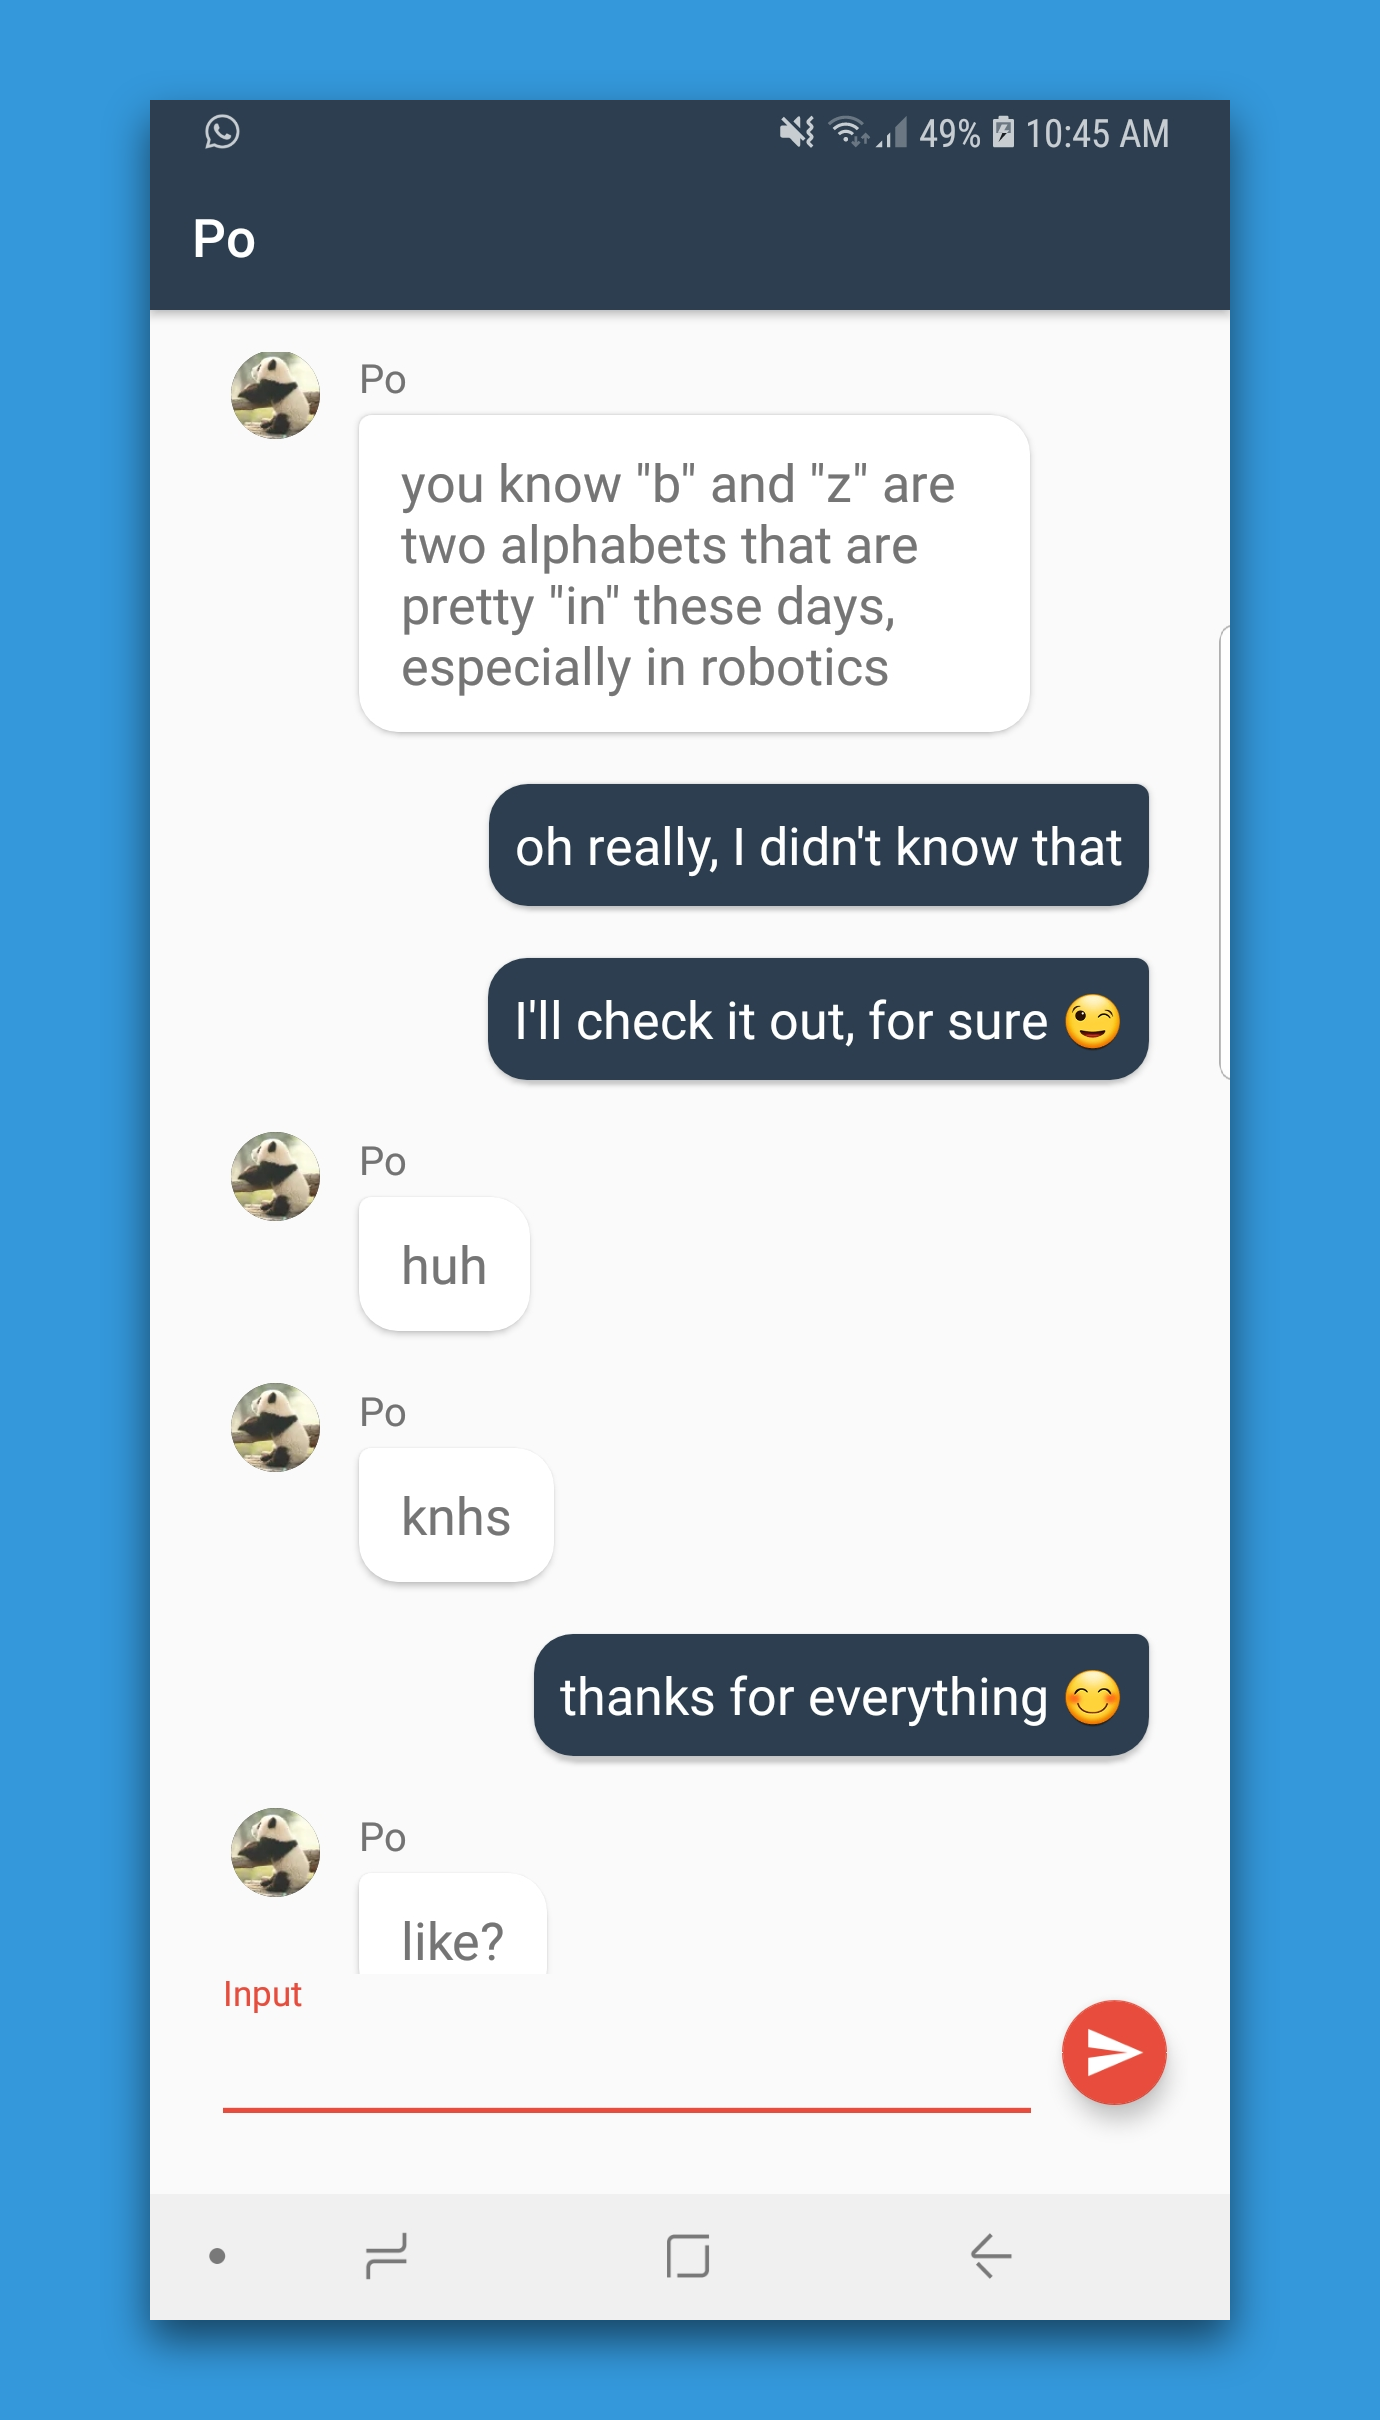
\includegraphics[width=0.80\textwidth]{images/khoji_chat.png}
	\caption{UI for real-time chatting in Khoji}
	\label{fig:khoji_chat}
\end{figure}


\section{Chat Bot Integration}
We have also included a chatbot in our application to aid the user in effectively using this app and to make his experience more enjoyable. The chatbot will be automatically added to the contacts of all the users as soon as they sign-up. The users could ask a simple question to the bot, and it will respond accordingly, doing his best to satisfy the needs of the users. The bot should be able to understand almost all of the queries of the user as it will use NLP (Natural Language Processing) to comprehend the user's queries.

Several options provided the services we required for our application, and among them, we chose \textbf{DialogFlow} \cite{DialogFlow2018} for this application. Formerly, this was known as \textbf{Api.ai}, but after its acquisition by Google, they changed its name to DialogFlow. We chose DialogFlow because of their fantastic documentation, easy customization and quick integration with several platforms. The main reason we went with DialogFlow is their pricing model \cite{DialogFlowPricing2018}. They provide free services in their Standard Edition plan, which has more than enough criteria for our app usage. 

\begin{figure}
    \centering
        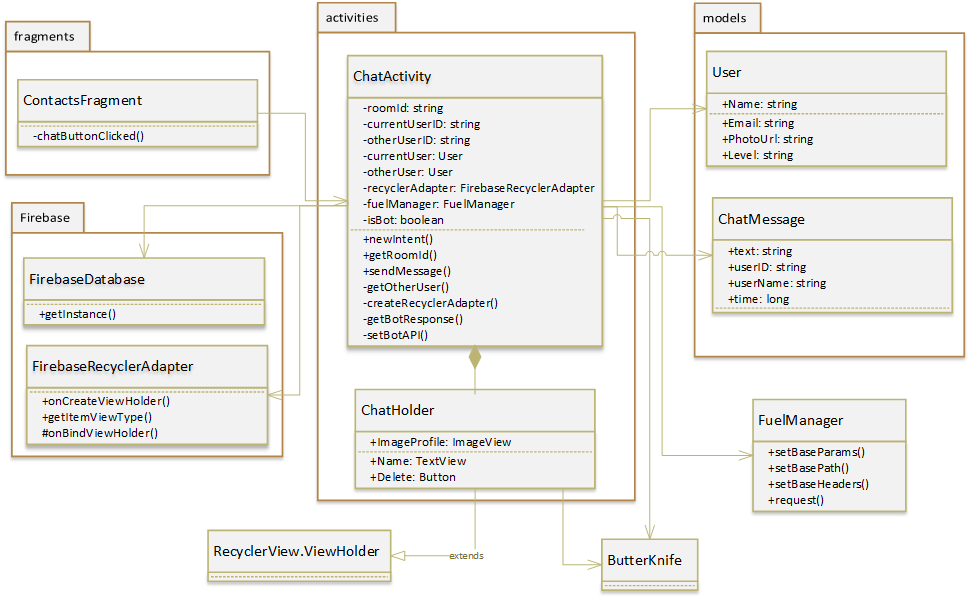
\includegraphics[width=1.00\textwidth]{images/uml-chat-bot.png}
    \caption{UML diagram for Chat Bot Integration}
    \label{fig:uml-chat-bot}
\end{figure}

As shown in Figure \ref{fig:uml-chat-bot}, we used Fuel to use the DialogFlow services. \texttt{Fuel} is a lightweight networking library that is used to send and retrieve requests across a network. We use \texttt{FuelManager} to call the REST services provided by DialogFlow to interact with our bot. The bot is trained on the DialogFlow platform using queries and answers specific to our application scenario. We then use FuelManager to send the query of the user from our app to the DialogFlow service, our bot receives the query and responds accordingly by sending the answer back to our application. 

When the ChatActivity is started, we first see if the user has initiated the chat with our Bot or not. If he is chatting with some other contact, nothing is changed, and it works just as before, but if he has initiated the chat with our Bot, we first set up the Bot API details, that is the credentials and path to our bot so that Fuel could access it. Now, when the user sends the message, we first send a request to the bot with the user's query and also, store it in the Firebase Database. We listen for the response from the Bot and upon receiving the response, we save it in the database and show the message to the user in the UI. In this way, he can interact with the Bot to resolve his queries.

By using this architecture, we can update and improve our bot without affecting the user's experience and without him, having to update the app again and again to get the latest version of the bot. We update and train the bot in the DialogFlow platform, and it gets updated for all the clients as they can call the updated bot using the same API as they were using before.

\begin{figure}[H]
	\centering
		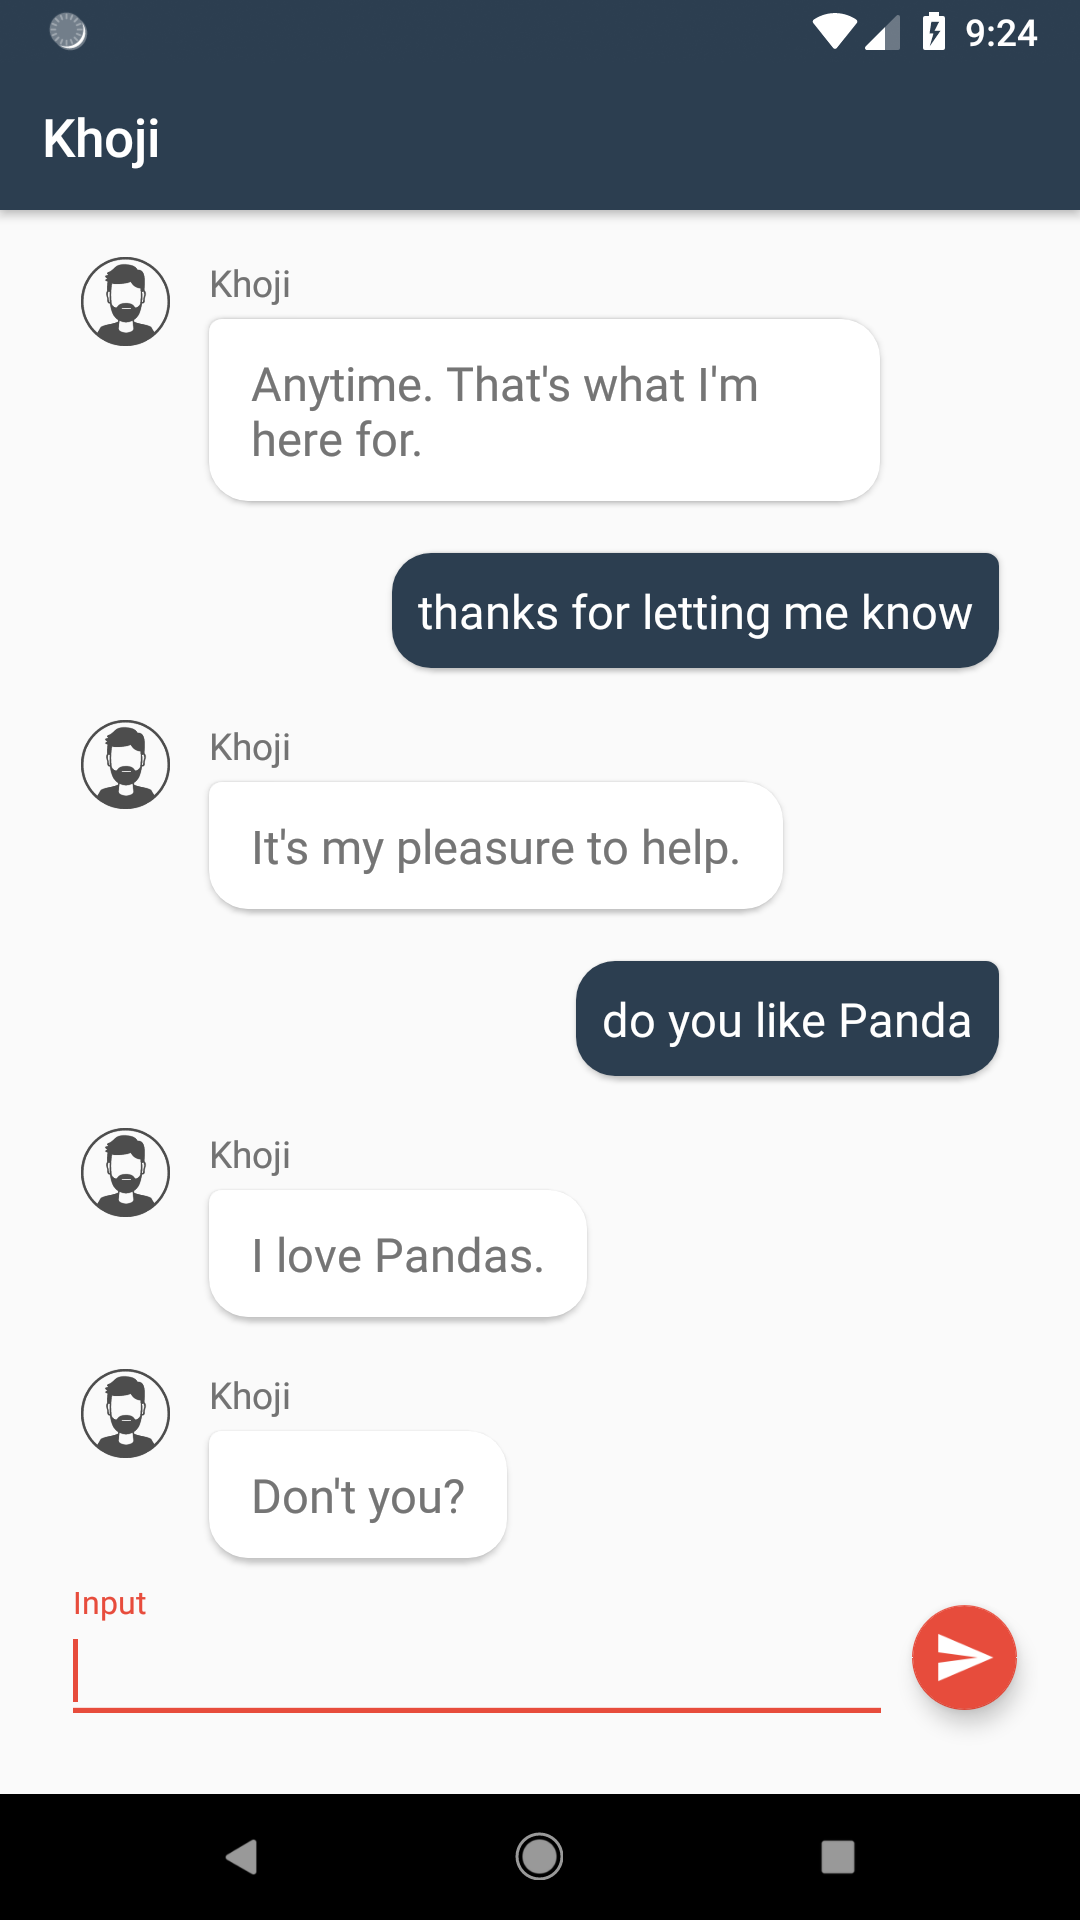
\includegraphics[width=0.80\textwidth]{images/khoji_chatbot.png}
	\caption{UI for Chat bot in Khoji}
	\label{fig:khoji_chatbot}
\end{figure}








